\begin{figure}[h]
\centering
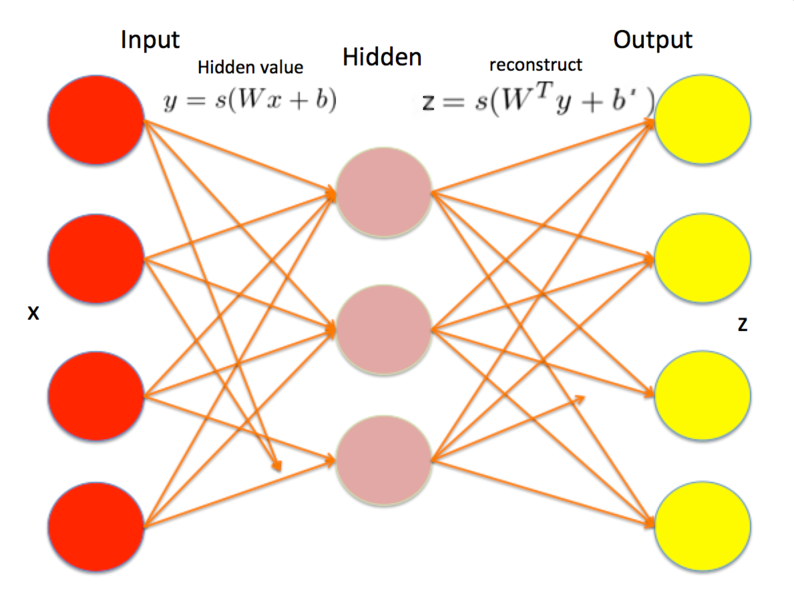
\includegraphics[width=0.8\linewidth]{autoencoder.png}
\caption{Overview of an autoencoder and its encoding, decoding stages. The weight matrix of the decoding stage is the transpose of the weight matrix of the encoding stage.}
\label{fig:autoencoder}
\end{figure}

Autoencoders are a method for performing representation learning, an unsupervised pretraining process during which a more useful representation of the
input data is automatically determined. Representation learning is important in machine learning since ``the performance of 
machine learning methods is heavily dependent on the choice of data representation (or features) in which they are applied" 
\cite{bengio2012rep}. For many supervised classification tasks, the high dimensionality of the input data means that the classifier requires an enormous number of training examples in order to generalize well and not overfit. One solution is to use unsupervised pretraining to learn a good representation for the input data and during actual training, transform the input examples into an easier form for the classifier to learn. Autoencoders are one such representation learning tool.

An autoencoder is a neural network with a single hidden layer and where the output layer and the input layer have the same size. Suppose that the input $x\in\mathbb{R}^m$ (and the output as well) and suppose that the hidden layer has $n$ nodes. Then we have a weight matrix $W\in\mathbb{R}^{m\times n}$ and bias vectors $b$ and $b^{'}$ in $\mathbb{R}^m$ and $\mathbb{R}^n$, respectively. Let $s(x) = 1/(1+e^{-x})$ be the sigmoid (logistic) transfer function. Then we have a neural network as shown in Fig.~\ref{fig:autoencoder}. When using an autoencoder to encode data, we calculate the vector $y=s(Wx + b)$; corresponding when we use an autoencoder to decode and reconstruct back the original input, we calculate $z=s(W^{T}x+b^{'})$. The weight matrix of the decoding stage is the transpose of weight matrix of the encoding stage in order to reduce the number of parameters to learn. We want to optimize $W$, $b$, and $b^{'}$ so that the reconstruction is as similar to the original input as possible with respect to some loss function. In this report, the loss function used is the least squares loss: $E(t,z)=\frac{1}{2}\norm{t-z}_2^2$, where $t$ is the original input. After an autoencoder is trained, its decoding stage is discarded and the encoding stage is used to transform the training input examples as a preprocessing step. We will refer to the trained encoding stage of the autoencoder as an ``autoencoder layer".

Once an autoencoder layer has been trained, a second autoencoder can be trained using the output of the first autoencoder layer. This procedure can be repeated indefinitely and create stacked autoencoder layers of arbitrary depth. It is been shown that each subsequent trained layer learns a better representation of the output of the previous layer. Using deep neural networks such as stacked autoencoders to do representation learning is also called deep learning, a subfield of machine learning that has received much attention and breakthroughs lately. 

For ordinary autoencoders, we usually want that $n<m$ so that the learned representation of the input exists in a lower dimensional space than the input. This is done to ensure that the autoencoder does not learn a trivial identity transformation. However, there also exists an autoencoder variant called \textit{denoising autoencoders} that use a different reconstruction criterion to learn overcomplete representations \cite{vincent2010stacked}. In other words, even if $n>m$, a denoising autoencoder can still learn a good representation of the input. This is achieved by corrupting the input image and training the autoencoder to reconstruct the original uncorrupted image. By learning how to denoise, the autoencoder is forced to understand the true structure of input data and learn a good representation of it. Although the loss function $E(t,z)$ for neural networks in general is non-convex, past work has shown that stochastic gradient descent (SGD) is sufficient for most problems. In this report, we will consider training denoising autoencoders with SGD. 

Lastly, we will examine training autoencoders with other optimization methods such as a genetic algorithm (GA). A GA is a biologically inspired black-box optimization algorithm is capable of optimizing arbitrary non-convex, non-differential objective functions. The motivations behind using GAs for training autoencoders are two fold: 1) GAs are a novel approach to optimization of deep neural networks with large number of parameters such as autoencoders. We would like to evaluate the performance of GAs and compare it to SGD. 2) GAs have some advantages over SGD such as being able to escape local optimas and easier to parallelize. However GAs also have drawbacks, the main one being its computational complexity over gradient descent. Unlike SGD, a GA must keep a population of individuals and must evaluate each individual for each training example. The computational complexity of a GA is $O(mnd)$ where $d$ is the dimensionality of the individual and objective function, $n$ is the population size, and $m$ is the number of training examples; in comparison, the complexity of SGD is $O(md)$. The optimal population size depends on the problem being solved, but in most cases, $n=O(d)$. 

We will not just implement a conventional GA (CGA), but also explore hybrid GAs that also make use of gradient information (HGA). The key idea is that with additional gradient information to intelligently update the population every generation, the population size can be kept constant. As a result, the complexity of HGA becomes the same as SGD: $O(md)$, while still retaining the advantages of being more scalable and capable of optimizing arbitrary objective functions.

The rest of this report is as follows: Past research and background literature for autoencoders, dimensionality reduction, genetic algorithms, representation and deep learning can be found in the related work section. The algorithm description section contains more details about how SGD, CGA, and HGA are implemented for autoencoders. The experiments section describes the performance of SGA, CGA, and HGA, as well as the results of training an autoencoder on a handwritten digit image dataset. In the discussion section, we will analyze our findings and report key findings. Finally, in future work, we discuss possible areas of future research.  




